\documentclass{article}
\usepackage[utf8]{inputenc}
\usepackage[margin=1.2in]{geometry}
\usepackage{graphicx}
\usepackage{xcolor}
\usepackage{listings}
\usepackage{float}
\usepackage{subcaption}
\lstset{
  language=python,
  columns=fullflexible,
  frame=single,
  breaklines=true,
  moredelim=**[is][\color{red}]{@}{@}
}

\title{Machine Learning}
\author{Martin Guyard et Guillaume Brizolier}
\date{TP2 : Renewable Energy Prediction}

\begin{document}

\maketitle

\section{Introduction}
L’objectif du TP est de proposer des modèles d’apprentissage automatique sur des jeux de données resultsSolar.csv et resultsWind.csv qui sont des données de productions d’une entreprise fournisseur d’énergies alternatives. Pour chaque jeu de données il faut réaliser deux tâches : la reconstruction (prédiction au temps courant) et la prédiction (prédiction au temps futur), sur deux features différentes : 'System power generated (kW)' et 'Electricity load (year 1) (kW)'.

\section{Preprocessing des données}
Avant de proposer des modèles, il faut s'assurer que les données d'apprentissage respectent certaines conditions. La nature des données d'apprentissage conditionne en grande partie les résultats obtenus. Nos modèles ne peuvent être satisfaisants qu'en regard des données avec lesquelles nous les nourissons, si les données sont indépendantes, variées, normalisées et correctement formatées, alors nous avons déjà une bonne base pour travailler un modèle d'apprentissage qui reponde à notre besoin (ie reconstruction d'une feature et prédiction d'une feature).

\subsection{Problèmes éventuels dans les données}
\begin{enumerate}
    \item Redondance : la redondance pose problème lorsque la target/cible est redondante dans les données d'apprentissage. C'est le cas dans notre TP. 'System power generated', 'Electricity load' et 'Bill load' sont redondantes. ('Bill load' est blacklisté)
    \item Normalisation : Il faut toujours normaliser pour des problèmes informatiques ! On soustrait la moyenne pour centrer les données puis on divise chaque colonne par la valeur max.
    \item Indépendance : fortement lié à la redondance. Dans notre cas, ce n'est pas un problème. On présuppose souvent l'indépendance des données, car les bases théoriques des modèles le présuppose.
    \item Format : Utilisation de one-hot vector (vecteur à valeur binaire) pour convertir les time-stamp en vecteur de données numériques. 
    
     \begin{center}
    \begin{tabular}{c|c|c|c|c|c|c}
        0 & 0 & 0 & 1 & 0 & 0 & 0 
    \end{tabular} 
    \textit{représentation one-hot de jeudi}
    \end{center}
    On utilise pour le time-stamp, 4 one-hot vectors : un de 12 cases pour les mois, un de 31 pour les jours, un de 24 pour les heures, et un de 7 pour le jours de la semaine.
    \item Trous : Si on a des trous, on peut soit faire des moyennes pondérées en fonction de points suivants et précédents, ou tout simplement remplacer par la moyenne (nulle ici car nous avons normalisé les données).
    \end{enumerate}

\section{Reconstruction}
   La reconstruction consiste à prédire au temps courant la valeur d’une des features demandée en fonction de toutes les autres features disponibles. Pour cette tâche on peut proposer un réseau neuronal et un algorithme plus ``old school`` type régression linéaire ou SVR.\\\\Une des limites du One-Hot vector est la décorrélation temporelle des données, ce n’est pas nécessairement un problème dans notre cas. Comme la corrélation temporelle existe entre nos données (l’instant t+1 est nécessairement proche de l’instant t, car les données sont des observations empiriques continues)\, il faut faire attention lors de l’apprentissage à donner à un ANN des ``observations successives`` dans le batch, pour l’entrainement et la validation. Par défaut ce nombre d’observations successives (chunk) est fixé à quelques heures.
   
    \subsection{Modèle régressif}
    Ce problème de prédiction pouvant s'assimiler à un problème de régression, nous avons choisi d'utiliser un SVR (\textit{Support Vector Regression}), importé depuis le module \textit{sklearn}.
    \begin{lstlisting}[frame=single]
        from sklearn.svm import SVR

        def model_no_ann(name, data, idx, target):
    """ Train a model on train + valid data set
    # Argument
        :param name: str, name
        :param data: numpy array, data
        :param idx: dict, data sets indexes
        :param target: int, position of target
    """
        fn = join(model_path, name)
        dt = np.concatenate((data[idx['train'], :target], data[idx['train'], target + 1:]), axis=-1)
        dv = np.concatenate((data[idx['valid'], :target], data[idx['valid'], target + 1:]), axis=-1)
        dtv = np.concatenate((dt, dv))
        ltv = np.concatenate((data[idx['train'], target], data[idx['valid'], target]))
        @model = SVR(epsilon=0.001)
        model.fit(dtv, ltv)@
        '''
        === Put some code here ===
        '''
        with open(fn, 'wb') as f:
            pidump(model, f)
        dtest = np.concatenate((data[idx['test'], :target], data[idx['test'], target + 1:]), axis=-1)
        @print("=====================Score : =====================")
        print(model.score(dtest, model.predict(dtest)))@
        graph_comparison([model.predict(dtest)], data, idx, target, 1, 0, t_idx='test', step=200)
    \end{lstlisting}
    Ici, le kernel utilisé est 'rbf' (paramètre par défaut) car les données ne sont pas linéairement séparables. On garde tous les autres paramètres à leur valeur par défaut, mis à part epsilon qu'on choisit à 0.001 pour un maximum de précision. Comme le montre les courbes de prédictions suivantes, le modèle prédit parfaitement les données de test, avec un model.score de 1.0, ce qui correspond d'après la documentation à un score parfait.
    \begin{figure}
        \centering
        \begin{subfigure}{.5\textwidth}
          \centering
          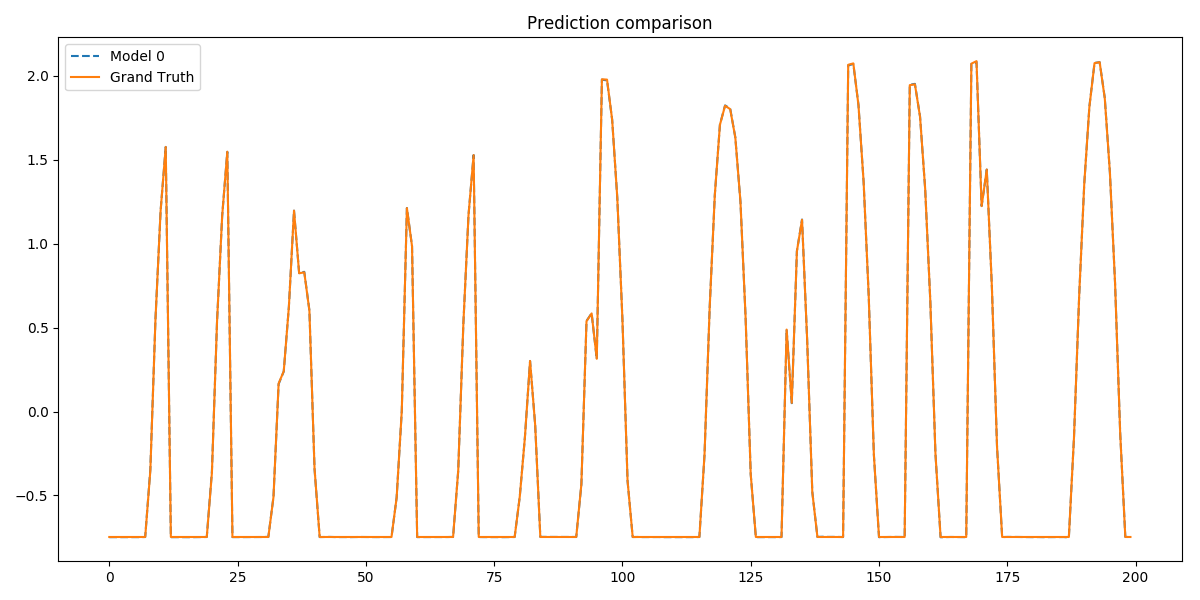
\includegraphics[scale=0.25]{ResultsSolar/comparison_test_0.png}
          \caption{Comparaison 1}
          \label{fig:sub1}
        \end{subfigure}%
        \begin{subfigure}{.5\textwidth}
          \centering
          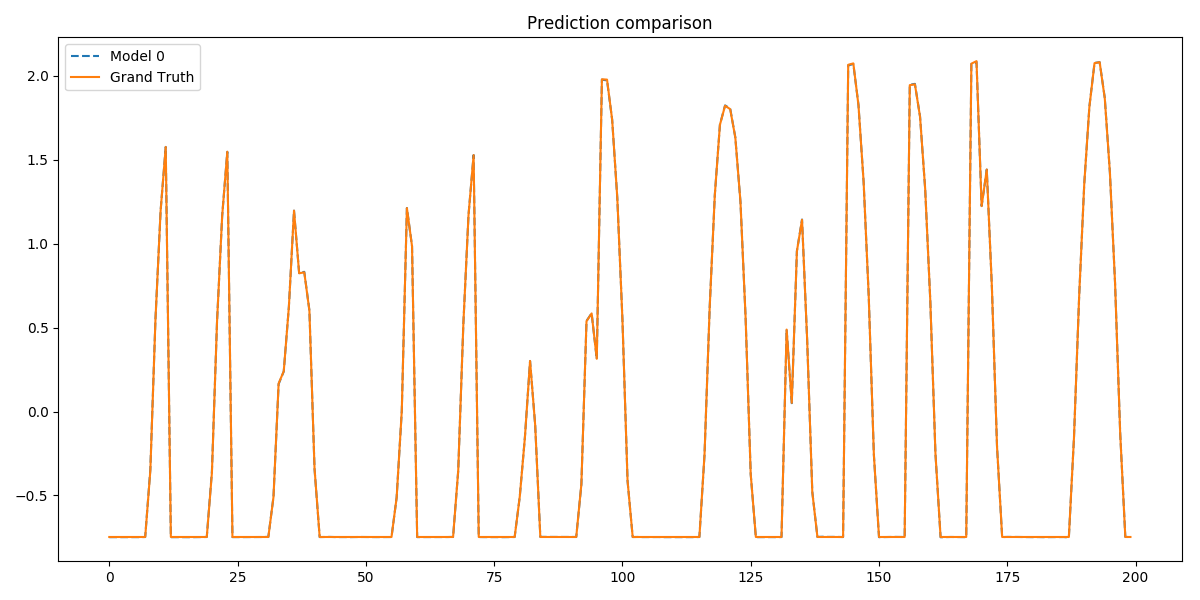
\includegraphics[scale=0.25]{ResultsSolar/comparison_test_0.png}
          \caption{Comparaison 2}
          \label{fig:sub2}
        \end{subfigure}
        \caption{Données d'apprentissage (orange solide) vs données prédites par le modèle (bleu pointillé)}
        \label{fig:test}
    \end{figure}
    Nous obtenons donc des performances très satisfaisantes pour ce modèle.
    \\\\\subsection{Modèle Réseau de Neurones}
    Nous tenons à préciser que tous les prochains exemples ont été obtenus sur le jeu de donnée resultsSolar.csv pour la feature System power generated.
    
    Nous avons choisi une architecture relativement simple pour notre réseau de neurones. Nous avons choisi de faire un ANN fully-connected, avec 3 couches 'dense' : la première avec 500 neurones, la deuxième avec 100, la troisième avec 10, complétée par une dernière couche d'une seule neurone sans fonction d'activation pour avoir le résultat final de la prédiction.\\\\Le code correspondant, écrit avec l'API fonctionnelle de Keras, est le suivant :\\
    \begin{lstlisting}[frame=single]
        def create_model(w, c):
        """ Create a keras model
        # Arguments
            :param w: int, time dimension
            :param c: int, channel dimension
        # Returns
            :return: keras model
        """
        l_in = Input(shape=(w, c,))  
        
        @l_hidden_0 = Dense(500, activation='relu')(l_in)
        l_hidden_1 = Dense(100, activation='relu')(l_hidden_0)
        l_hidden_2 = Dense(10, activation='relu')(l_hidden_1)
        l_hidden_3 = Dense(1)(l_hidden_2)@
        
        l_out = Flatten()(l_hidden_3)

        return Model(l_in, l_out)
    \end{lstlisting}

    On remarque qu'on utilise un layer Flatten au début. Cela est en fait dû aux différences de dimensions de l'input du modèle, qui doit correspondre aux dimensions données par les fonctions de générations de données, à savoir [batch, fenêtre, canaux], tandis que l'output lui correspond simplement à la dimension du batch.

    Les résultats pour ce modèle sont un peu moins convaincants, pour une raison que nous ne sommes pas arrivés à déterminer le modèle ne semble pas converger vers une valeur de loss satisfaisante.
    Voici les résultats que nous obtenons :\\
    \begin{figure}[H]
        \centering
        \begin{subfigure}[t]{0.49\textwidth}
            \raisebox{-\height}{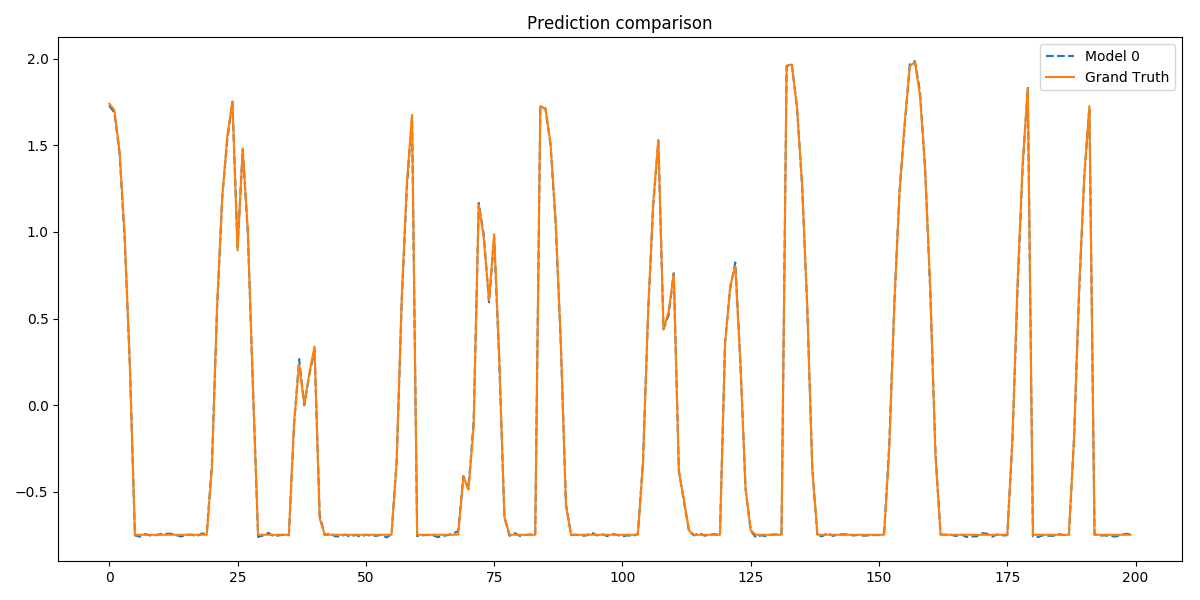
\includegraphics[width=\textwidth]{ResultsSolar/comparison_valid_0.png}}
            \caption{caption of first image}
        \end{subfigure}
        \hfill
        \begin{subfigure}[t]{0.49\textwidth}
            \raisebox{-\height}{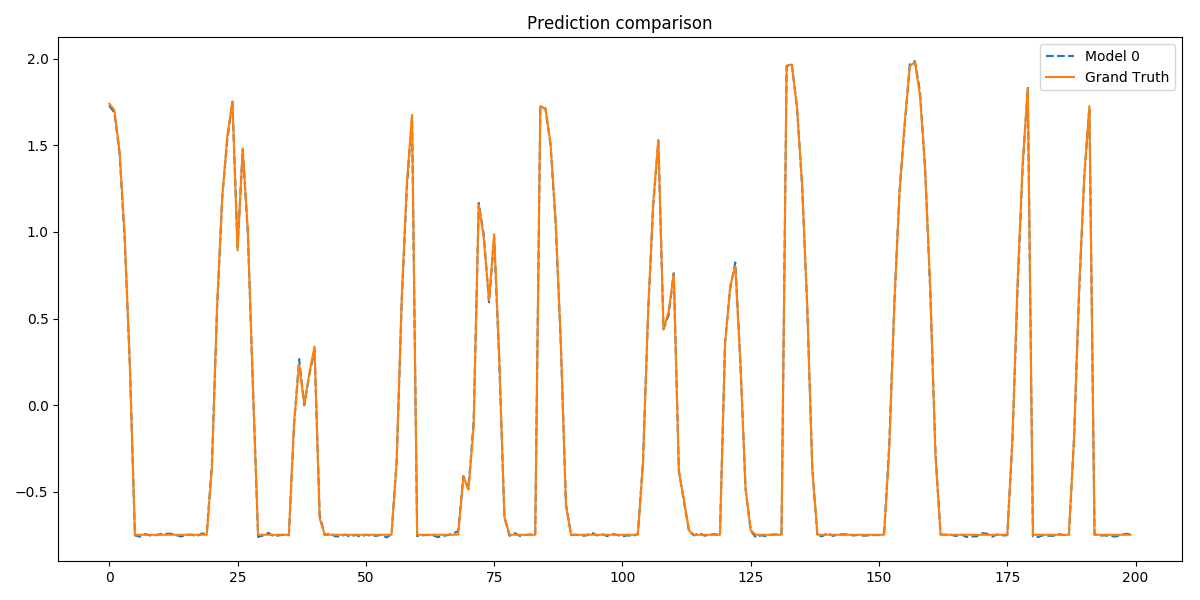
\includegraphics[width=\textwidth]{ResultsSolar/comparison_valid_0.png}}
        \caption{caption of second image\\second line}
    \end{subfigure}
        \caption{Données de validation (orange solide) vs données prédites par le modèle (bleu pointillé)}
        \label{fig:test}
    \end{figure}
    \begin{figure}[H]
        \centering
        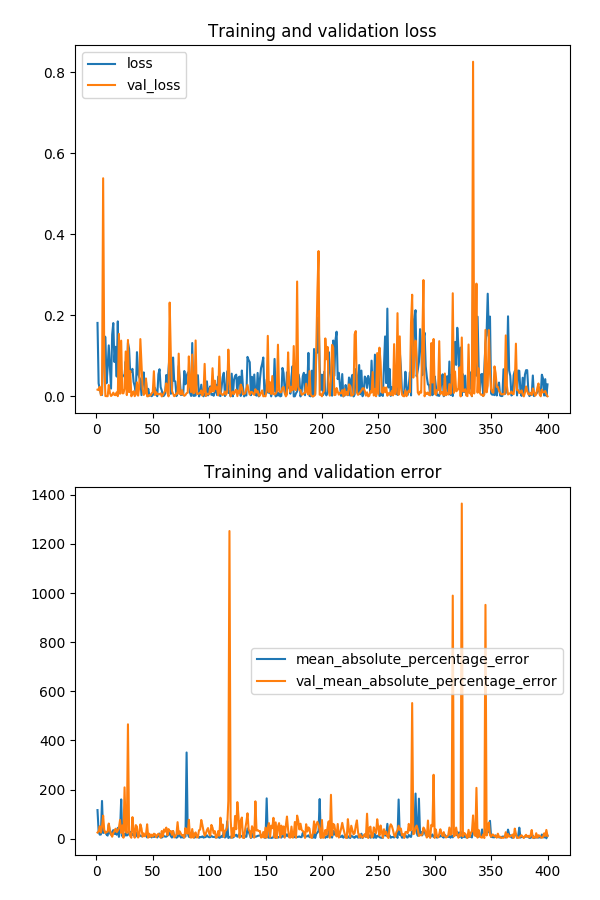
\includegraphics[scale=0.5]{ResultsSolar/results.png}
        \caption{Loss et Mean Squared Error en fonction du nombre d'epoch}
        \label{fig:schema}
    \end{figure}
    On observe que ni la minimisation de la loss (Train et Val) ni la minimisation de la métrique MAPE (Train et Val) ne sont stables.\\\\Il y a plusieurs méta-paramètres sur lesquels nous pouvons jouer, comme par exemple le nombre d'epoch (peu pertinent ici car pas d'indications claires de convergence), la taille des chunks, ou bien la taille du batch. Un paramètre important que l'on peut également modifier est le pas d'apprentissage. On peut aussi jouer sur les paramètres du réseau (nombre de couches, nombre de neurones par couches, fonctions d'activation).
    
    \begin{lstlisting}[frame=single]
        def create_model(w, c):
        """ Create a keras model
        # Arguments
            :param w: int, time dimension
            :param c: int, channel dimension
        # Returns
            :return: keras model
        """
        l_in = Input(shape=(w, c,))  
        
        @l_hidden_0 = Dense(400, activation='relu')(l_in)
        l_hidden_1 = Dense(200, activation='relu')(l_hidden_0)
        l_hidden_2 = Dense(100, activation='relu')(l_hidden_1)
        l_hidden_3 = Dense(50, activation='relu')(l_hidden_2)
        l_hidden_4 = Dense(10, activation='relu')(l_hidden_3)
        l_hidden_out = Dense(1, activation='linear')(l_hidden_4)@
        
        l_out = Flatten()(l_hidden_out)

        return Model(l_in, l_out)
    \end{lstlisting}
    Voici le nouveau réseau. On ne garde volontairement que des fonctions d'activation Relu, pour éviter des problèmes d'évanouissement du gradient du fait des 4 layers de notre modèle.\\\\On change également le chunk à 48 (heures) puis les méta-paramètres : epoch=200, lr=3e-5, batch=32, noise = None. En faisant plusieurs essais on se rend compte que le learning rate doit être correctement dimensionné pour assurer une convergence rapide (si trop petit pas/peu de convergence, si trop grand "rebonds" et pas de convergence non plus). Une fois le learning rate fixé on peut réaliser plusieurs essais en changeant les autres méta-paramètres. En diminuant la taille du batch, on perd évidemment en vitesse de calcul mais on gagne en précision sur la direction de diminution du gradient, donc on assure une meilleure convergence sur les minimas locaux de la fonction de loss.\\\\
    
     \begin{figure}[H]
        \centering
        \begin{subfigure}[t]{0.49\textwidth}
            \raisebox{-\height}{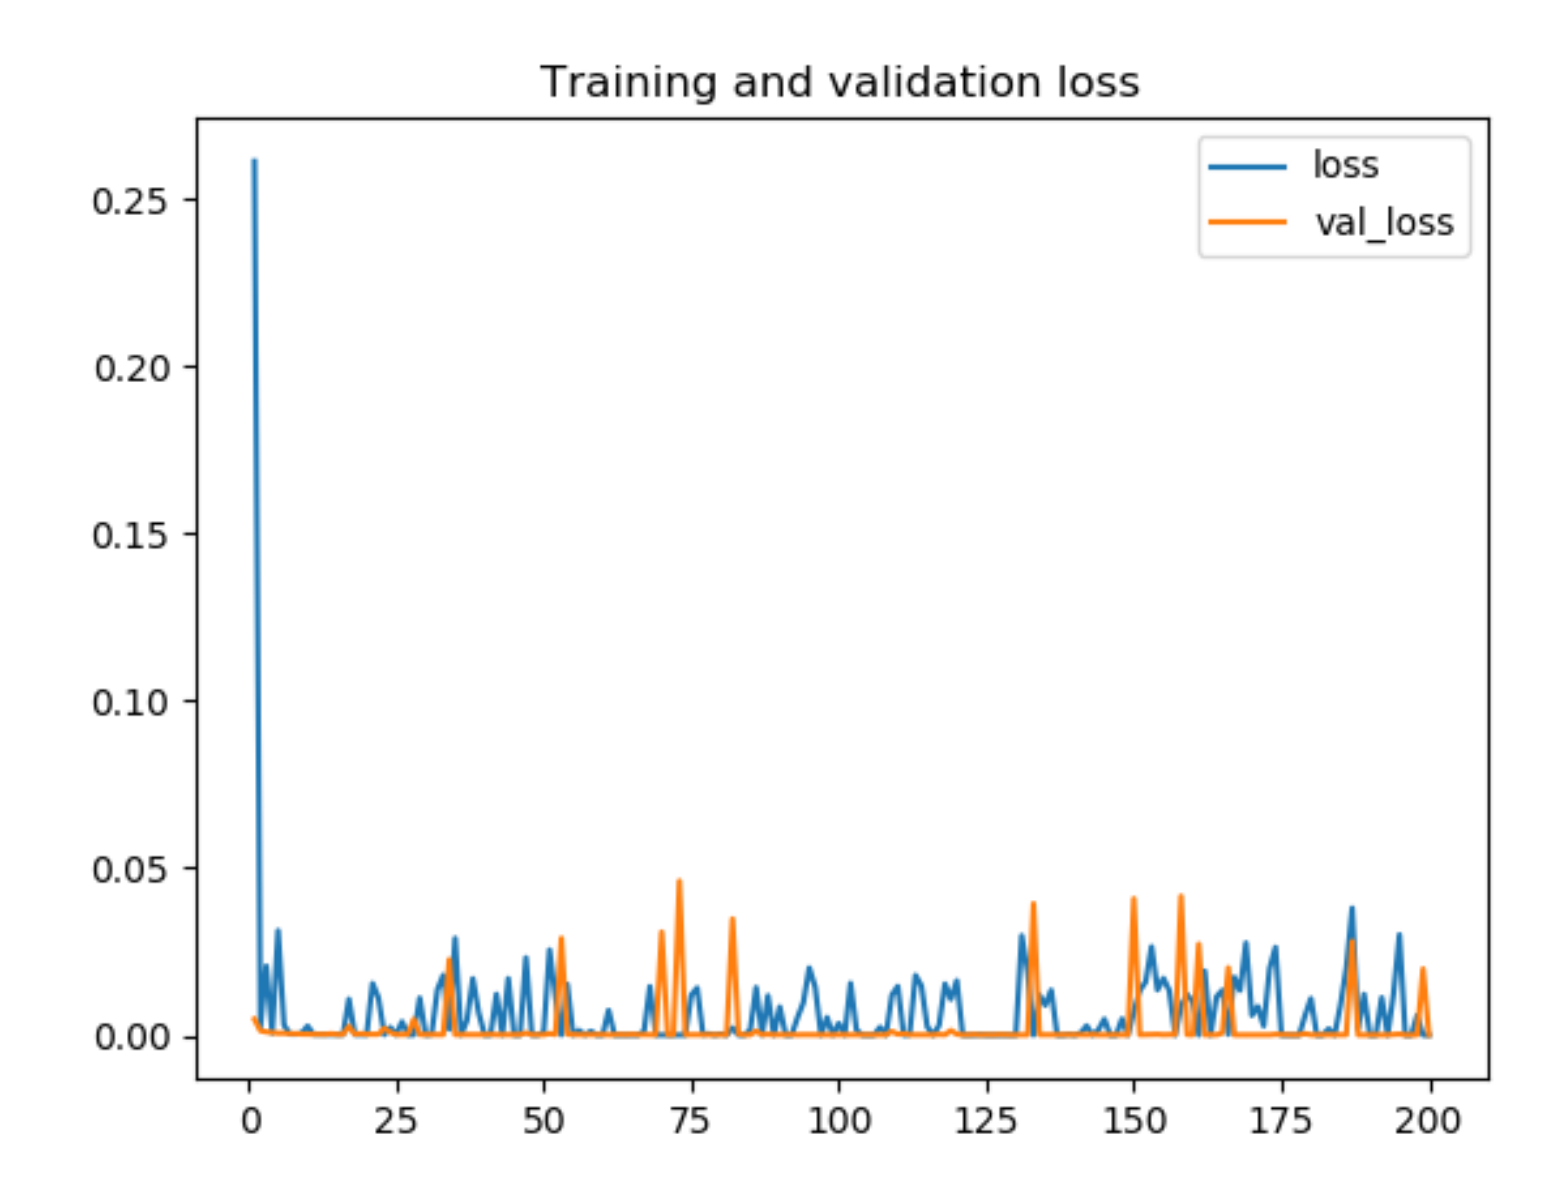
\includegraphics[width=\textwidth]{ResultsSolar/LogSolar11.png}}
            \caption{Minimisation de la Loss MSE}
        \end{subfigure}
        \hfill
        \begin{subfigure}[t]{0.49\textwidth}
            \raisebox{-\height}{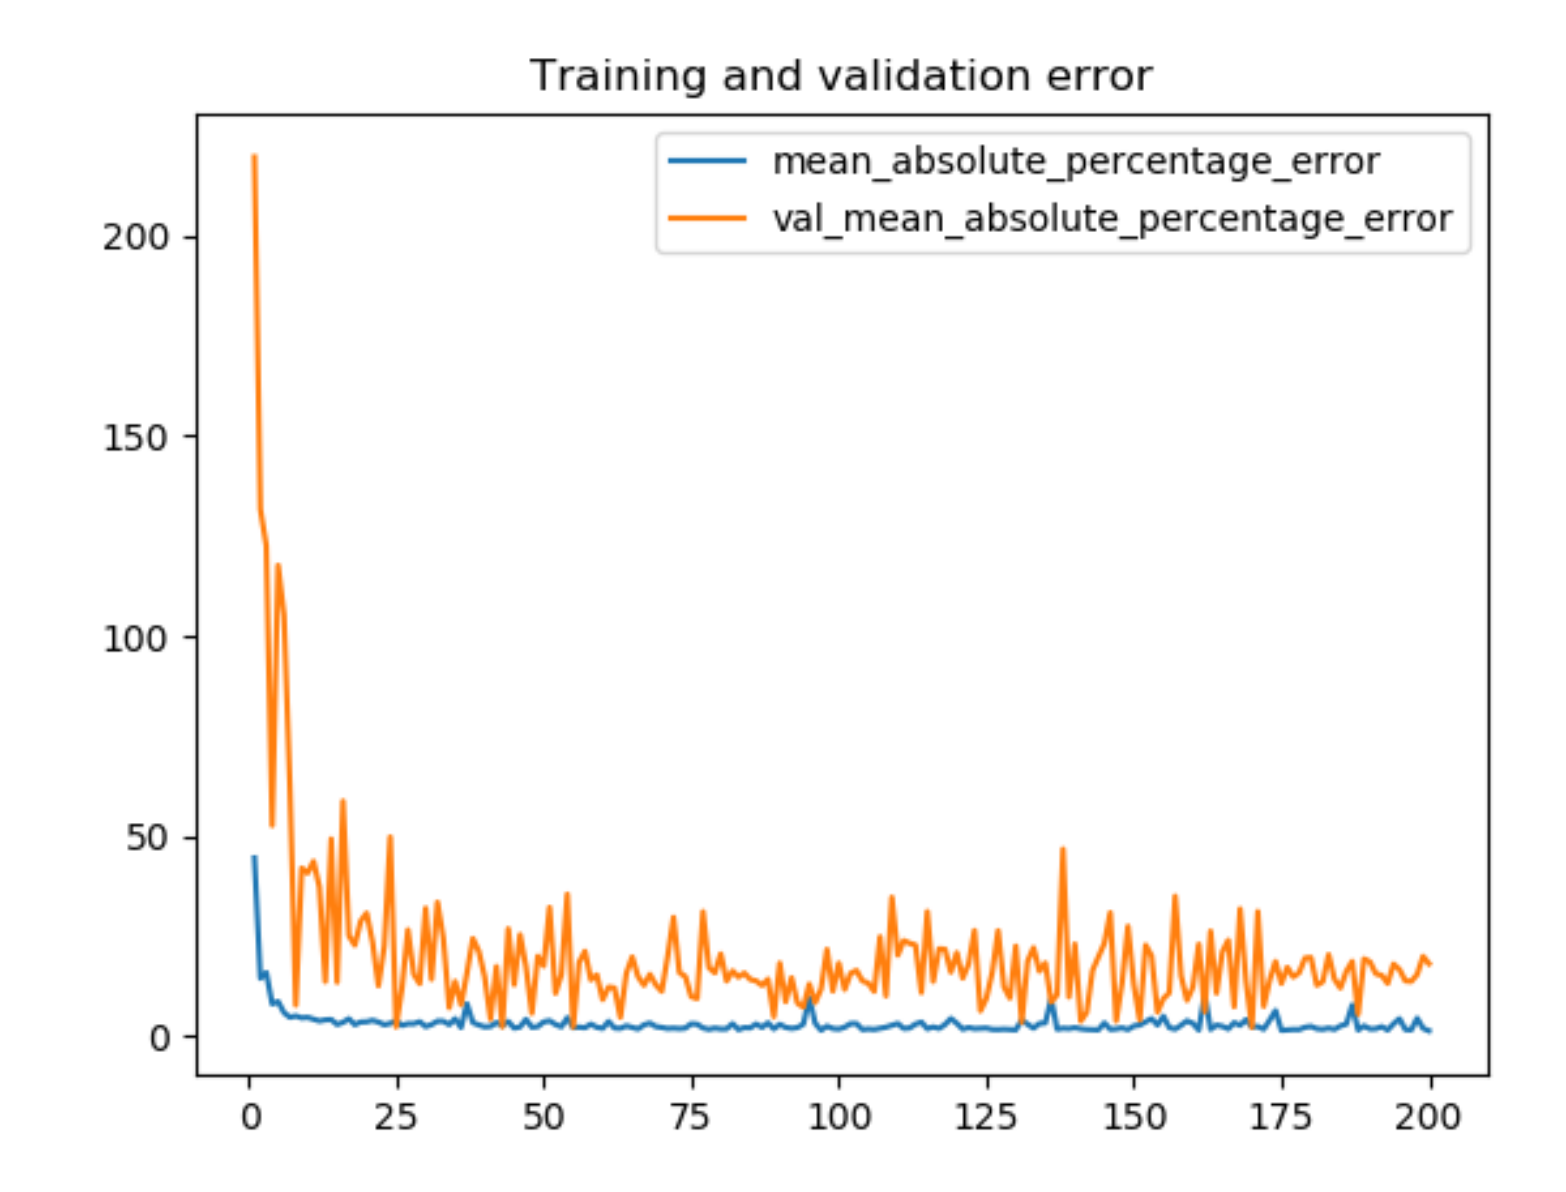
\includegraphics[width=\textwidth]{ResultsSolar/LogSolar12.png}}
        \caption{Métrique MAPE}
    \end{subfigure}
        \caption{Performance du réseau (Solar, System power generated)}
        \label{fig:test}
    \end{figure}
    
    Finalement la figure 4 montre une convergence satisfaisante vers un minimum  de la loss (MSE), des dataset Train et Val. Egalement on observe que la métrique (MAPE) des deux dataset converge et se stabilise. La remarque que l'on pourrait faire ici est que la métrique (MAPE) pour le dataset Val ne converge pas totalement vers la métrique (MAPE) du dataset Train, on peut soupçonnner un léger overfitting. On peut contrer cet overfitting en régularisant avec un peu de bruit : noise = 1e-5 (plus petit que le learning rate de préférence), en ajoutant un dropout, ou bien en reduisant la capacité du réseau (mais nous déconseillons cette option dans notre cas, car le réseau n'est pas particulièrement  complexe et qu'il répond assez bien à notre problème de minimisation).
    \\\\
    Nous proposons un dernier modèle pour cette partie, le réseau est inchangé, seuls les méta-paramètres sont modifiés. La taille du batch est multipliée par 2 et passe à 64, puis un bruit est ajouté pour améliorer la généralisation du réseau : epoch=200, lr=3e.5, noise=1e-5, batch=64.
    
    \begin{figure}[H]
        \centering
        \begin{subfigure}[t]{0.49\textwidth}
            \raisebox{-\height}{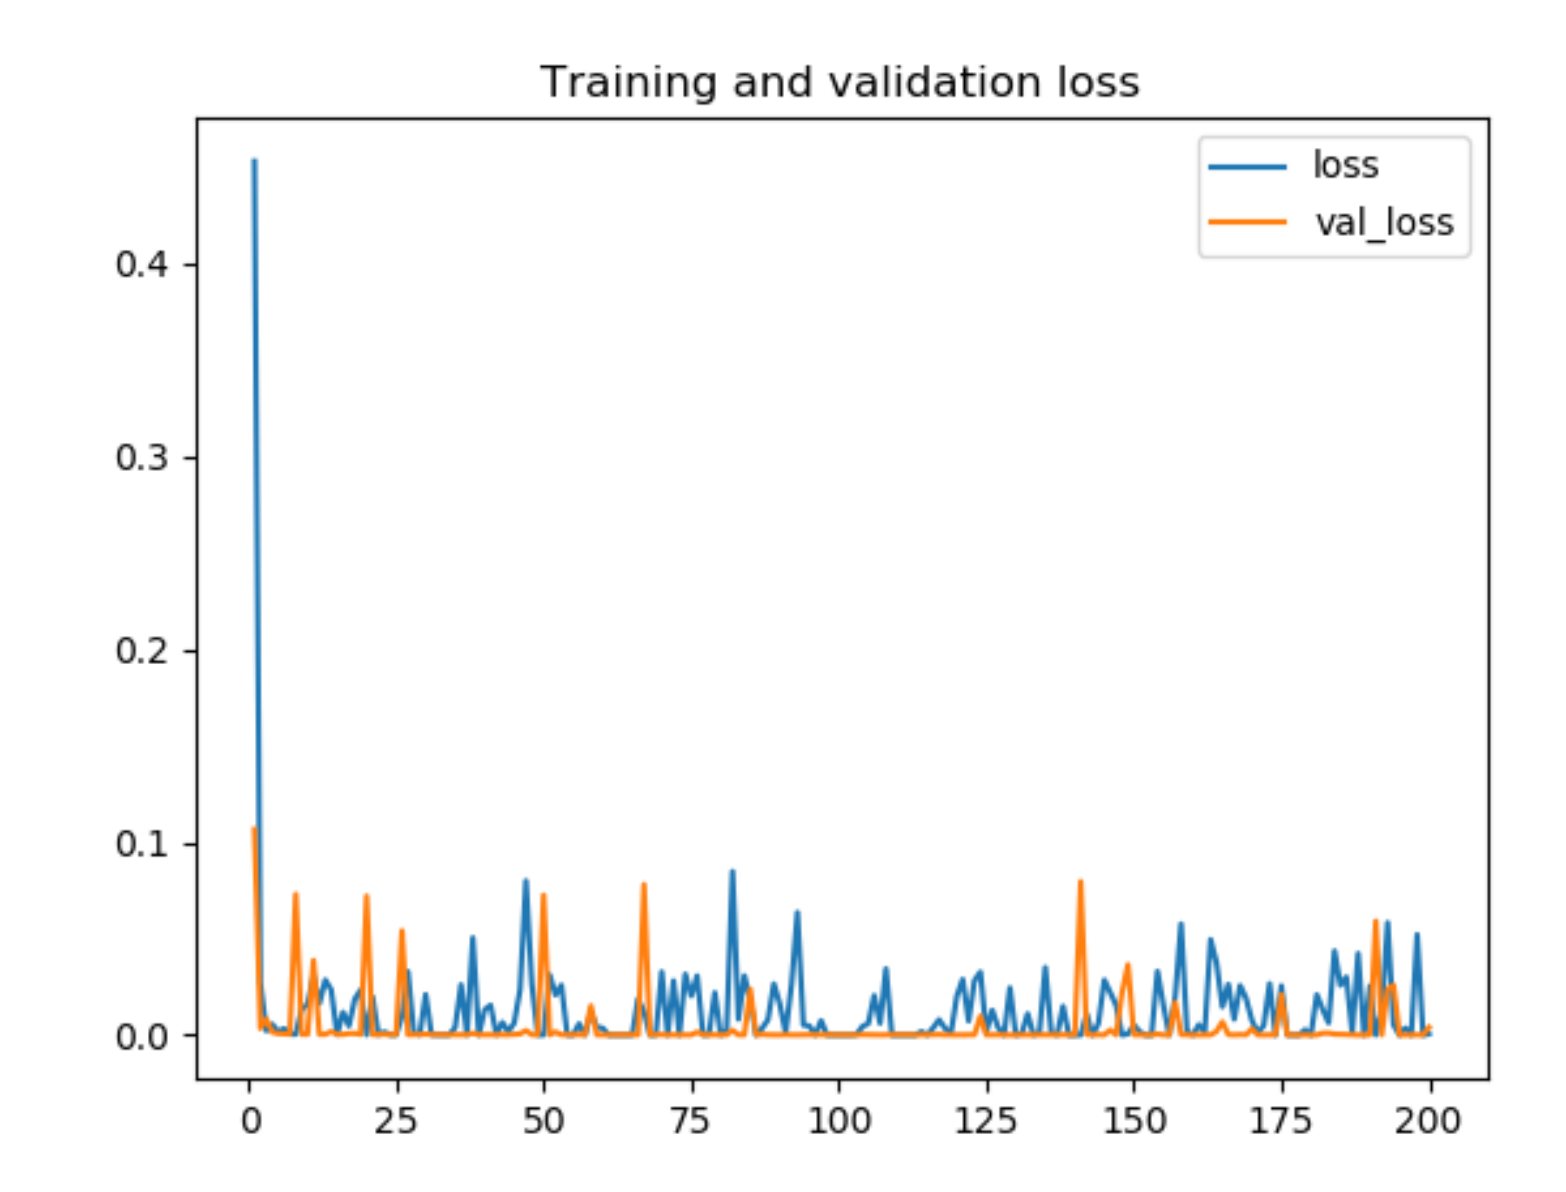
\includegraphics[width=\textwidth]{ResultsSolar/LogSolar21.png}}
            \caption{Minimisation de la Loss MSE}
        \end{subfigure}
        \hfill
        \begin{subfigure}[t]{0.49\textwidth}
            \raisebox{-\height}{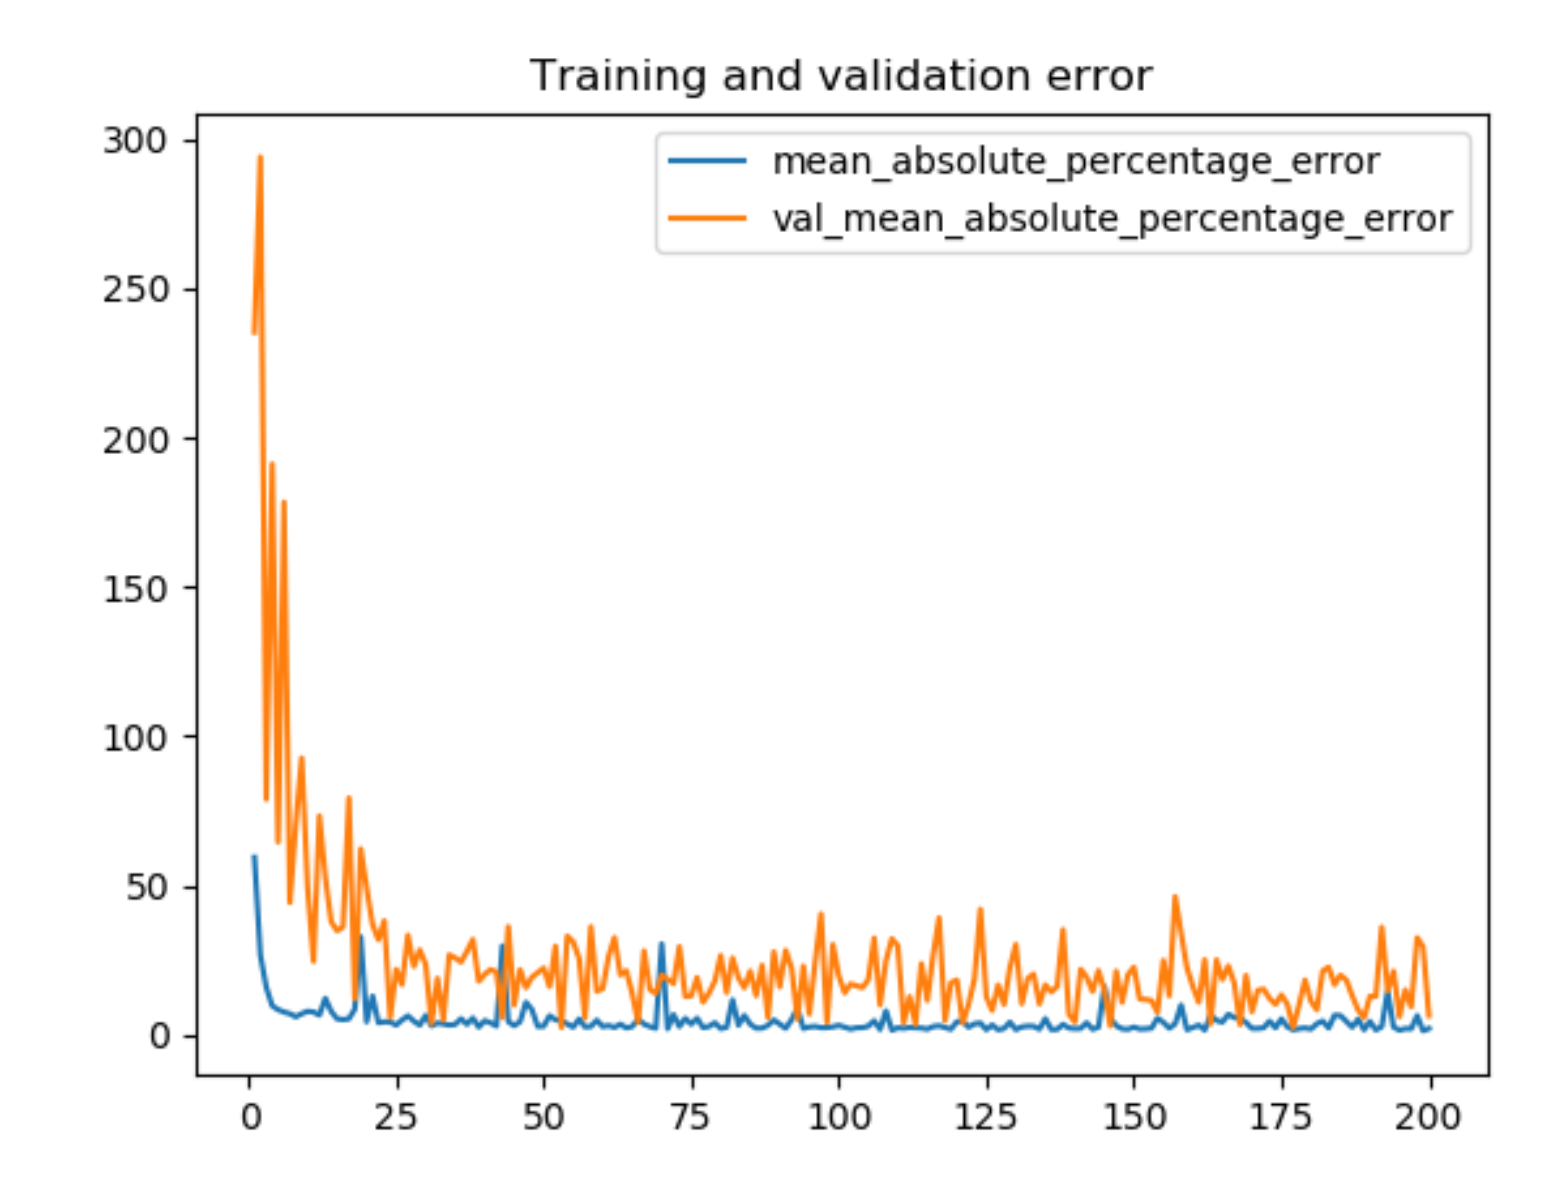
\includegraphics[width=\textwidth]{ResultsSolar/LogSolar22.png}}
        \caption{Métrique MAPE}
    \end{subfigure}
        \caption{Performance du réseau : Reconstruction (Solar, System power generated)}
        \label{fig:test}
    \end{figure}
    
    On voit bien une légère amélioration de la performance. L'erreur (métrique MAPE) du dataset de validation converge mieux vers la métrique du dataset Train : le réseau généralise suffisamment. On arrive à ce resultat en changeant les méta-paramètres d'apprentissage du réseau et non pas le réseau en lui même. Les prédictions réalisées sont très proches du "ground truth". C'est un des meilleur modèles que nous avons réalisé avec ce jeu de données.
    
    \begin{figure}[H]
        \centering
        \begin{subfigure}[t]{0.49\textwidth}
            \raisebox{-\height}{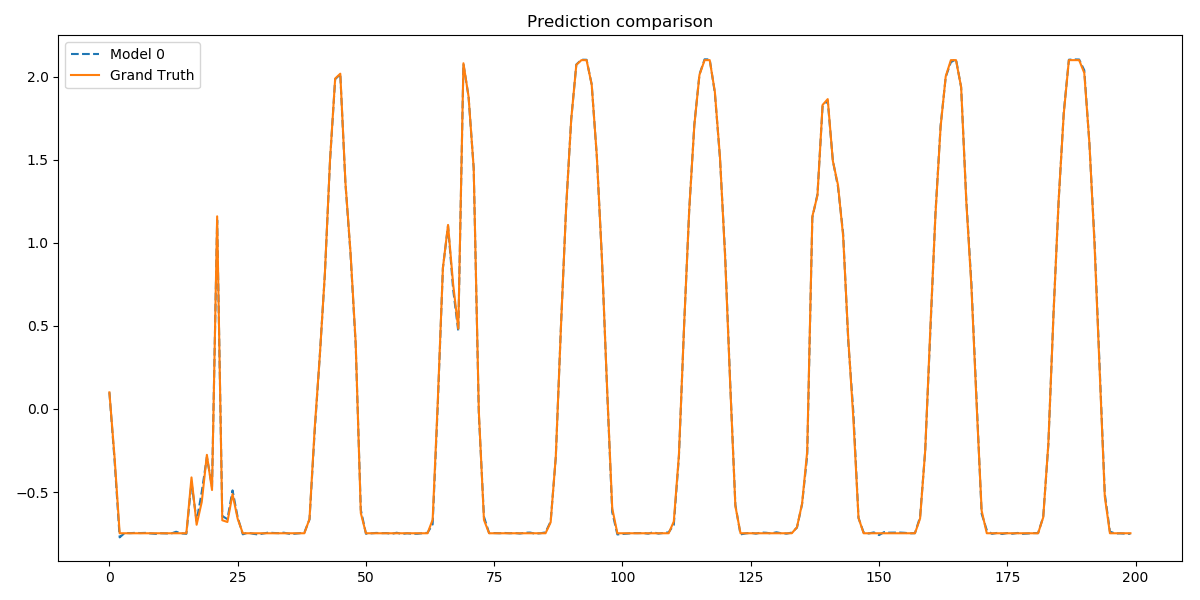
\includegraphics[width=\textwidth]{ResultsSolar/Solar_test.png}}
            \caption{Comparaison Test}
        \end{subfigure}
        \hfill
        \begin{subfigure}[t]{0.49\textwidth}
            \raisebox{-\height}{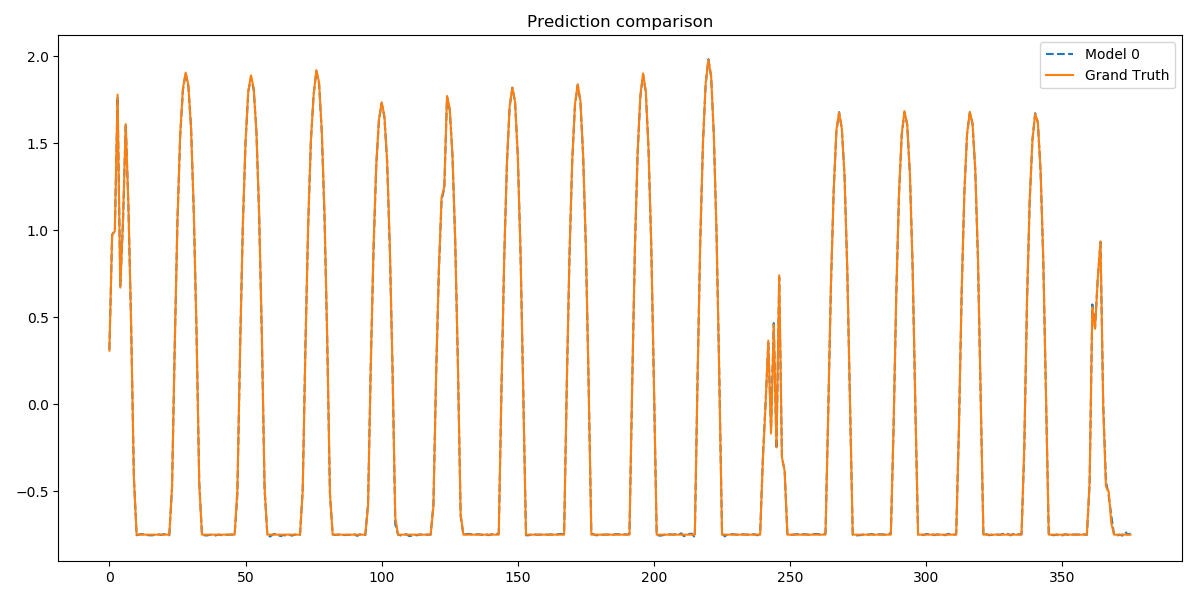
\includegraphics[width=\textwidth]{ResultsSolar/Solar_validation.png}}
        \caption{Comparaison Valid}
    \end{subfigure}
        \caption{Ecart de prédiction : Reconstruction (Solar, System power generated)}
        \label{fig:test}
    \end{figure}
    
    En dernier exemple on applique un réseau similaire au jeu de données resultsWind.csv avec comme target la feature ``Electricity Load``.\\On observe ce que l'on suppose être un overffiting. En effet, la loss est bien minimisée mais la métrique MAPE des dataset Train et Val semble diverger.
    epoch=200, lr=1e-5, noise=3e-6, batch=64
    \begin{figure}[H]
        \centering
        \begin{subfigure}[t]{0.49\textwidth}
            \raisebox{-\height}{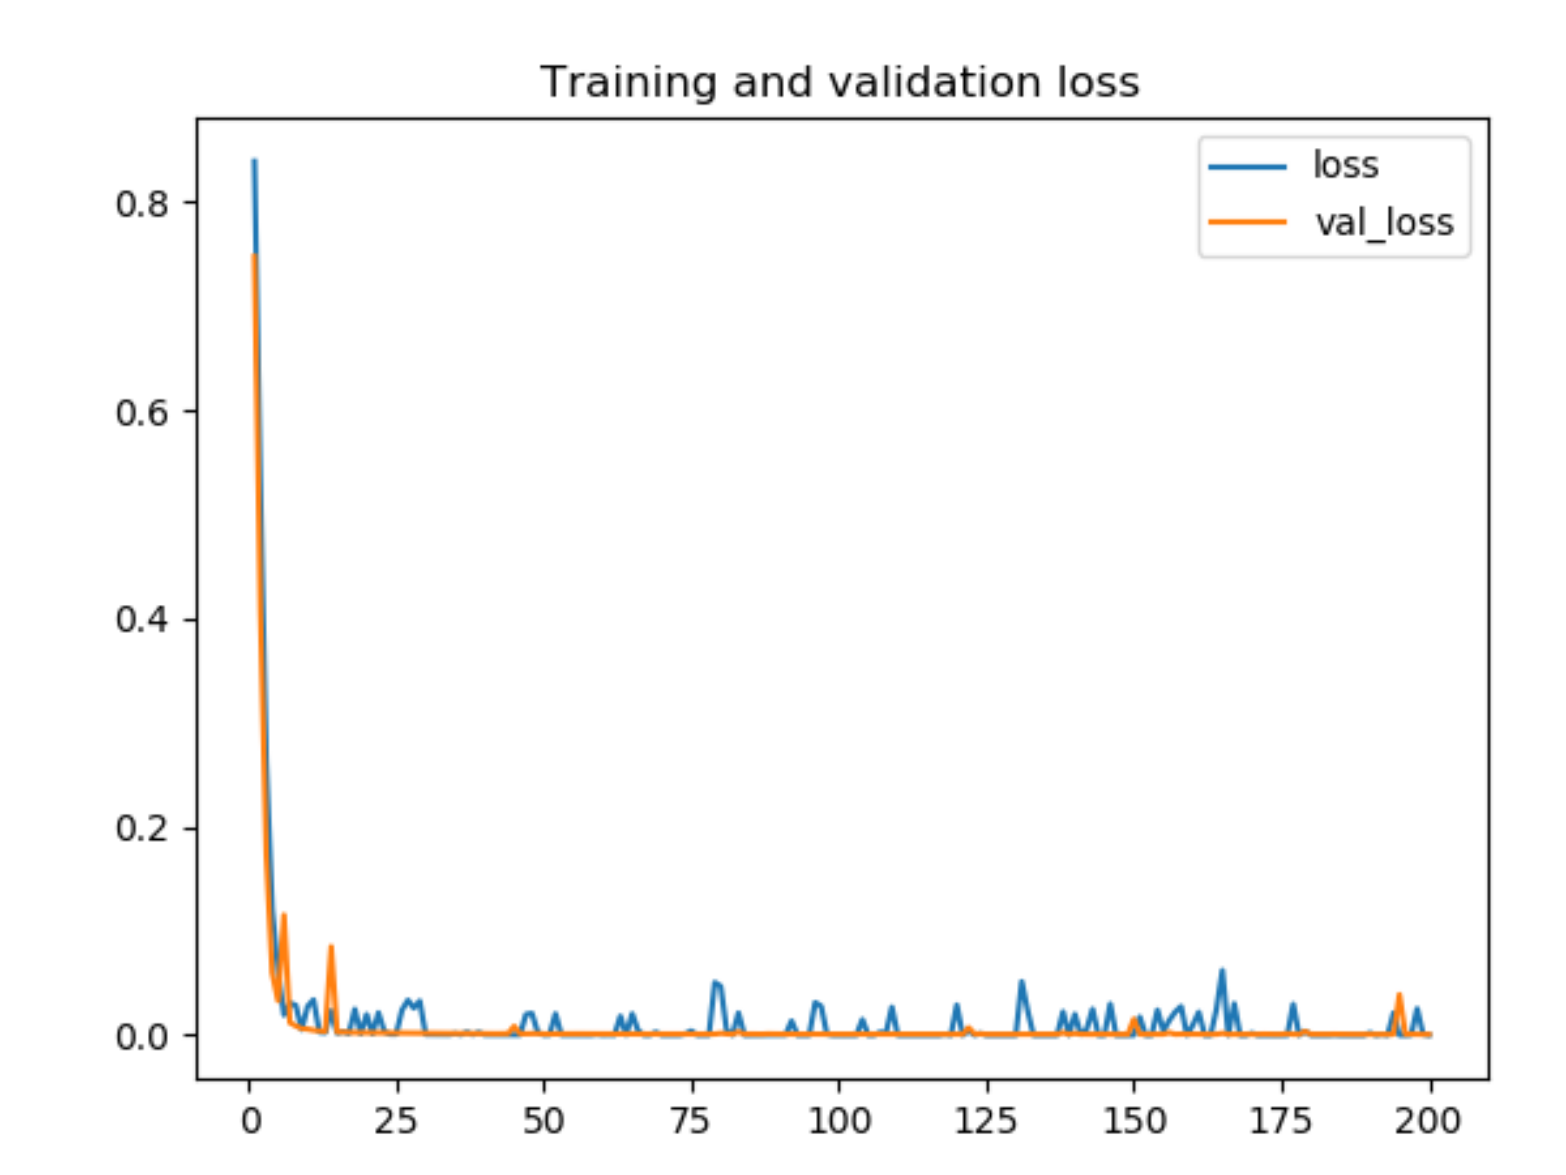
\includegraphics[width=\textwidth]{ResultsWind/WindLog11.png}}
            \caption{Minimisation de la Loss MSE}
        \end{subfigure}
        \hfill
        \begin{subfigure}[t]{0.49\textwidth}
            \raisebox{-\height}{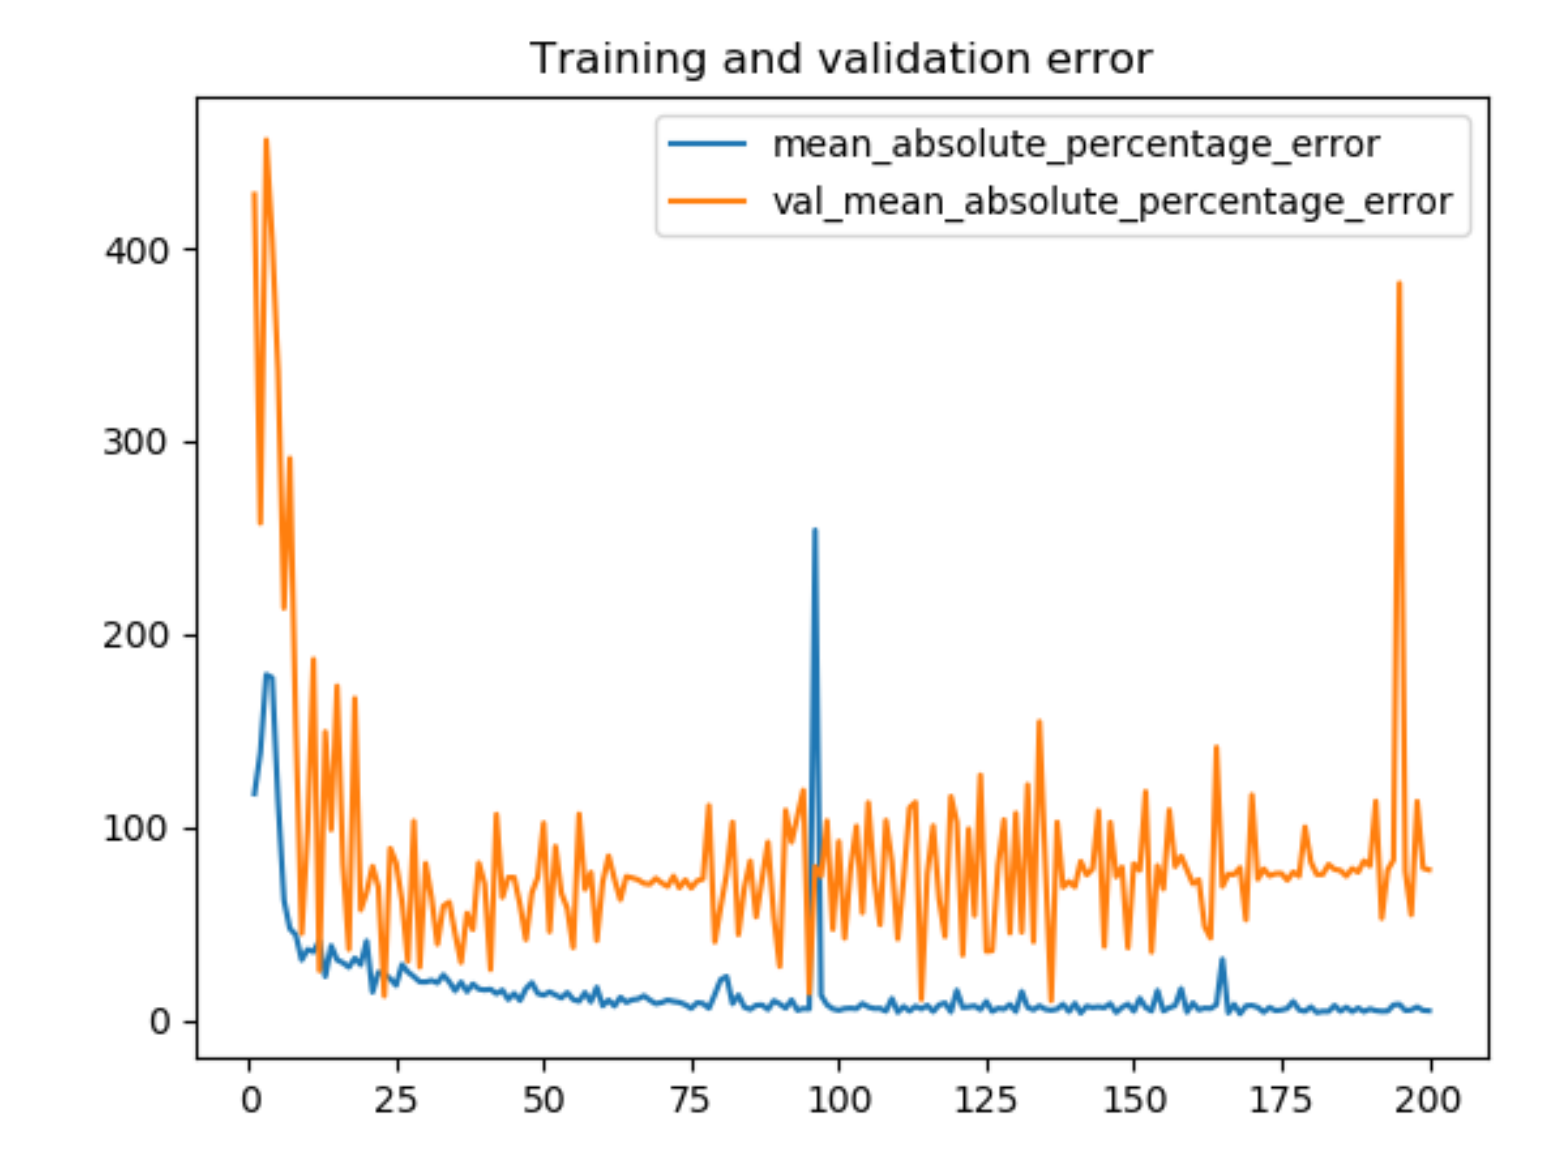
\includegraphics[width=\textwidth]{ResultsWind/Windlog12.png}}
        \caption{Métrique MAPE}
    \end{subfigure}
        \caption{Performance du réseau : Reconstruction (Wind, Electricity Load)}
        \label{fig:test}
    \end{figure}
    On modifie légèrement les méta-paramètres, epoch=300, lr=1e-6, noise=3e-7, batch=25 et chunk=50. On obtient un résultat légèrement meilleur car on vient de diminuer la divergence des métriques MAPE entre les dataset Train et Val. Egalement la minimisation de la loss pour les dataset Train et Val convergent mieux vers 0.
    \begin{figure}[H]
        \centering
        \begin{subfigure}[t]{0.49\textwidth}
            \raisebox{-\height}{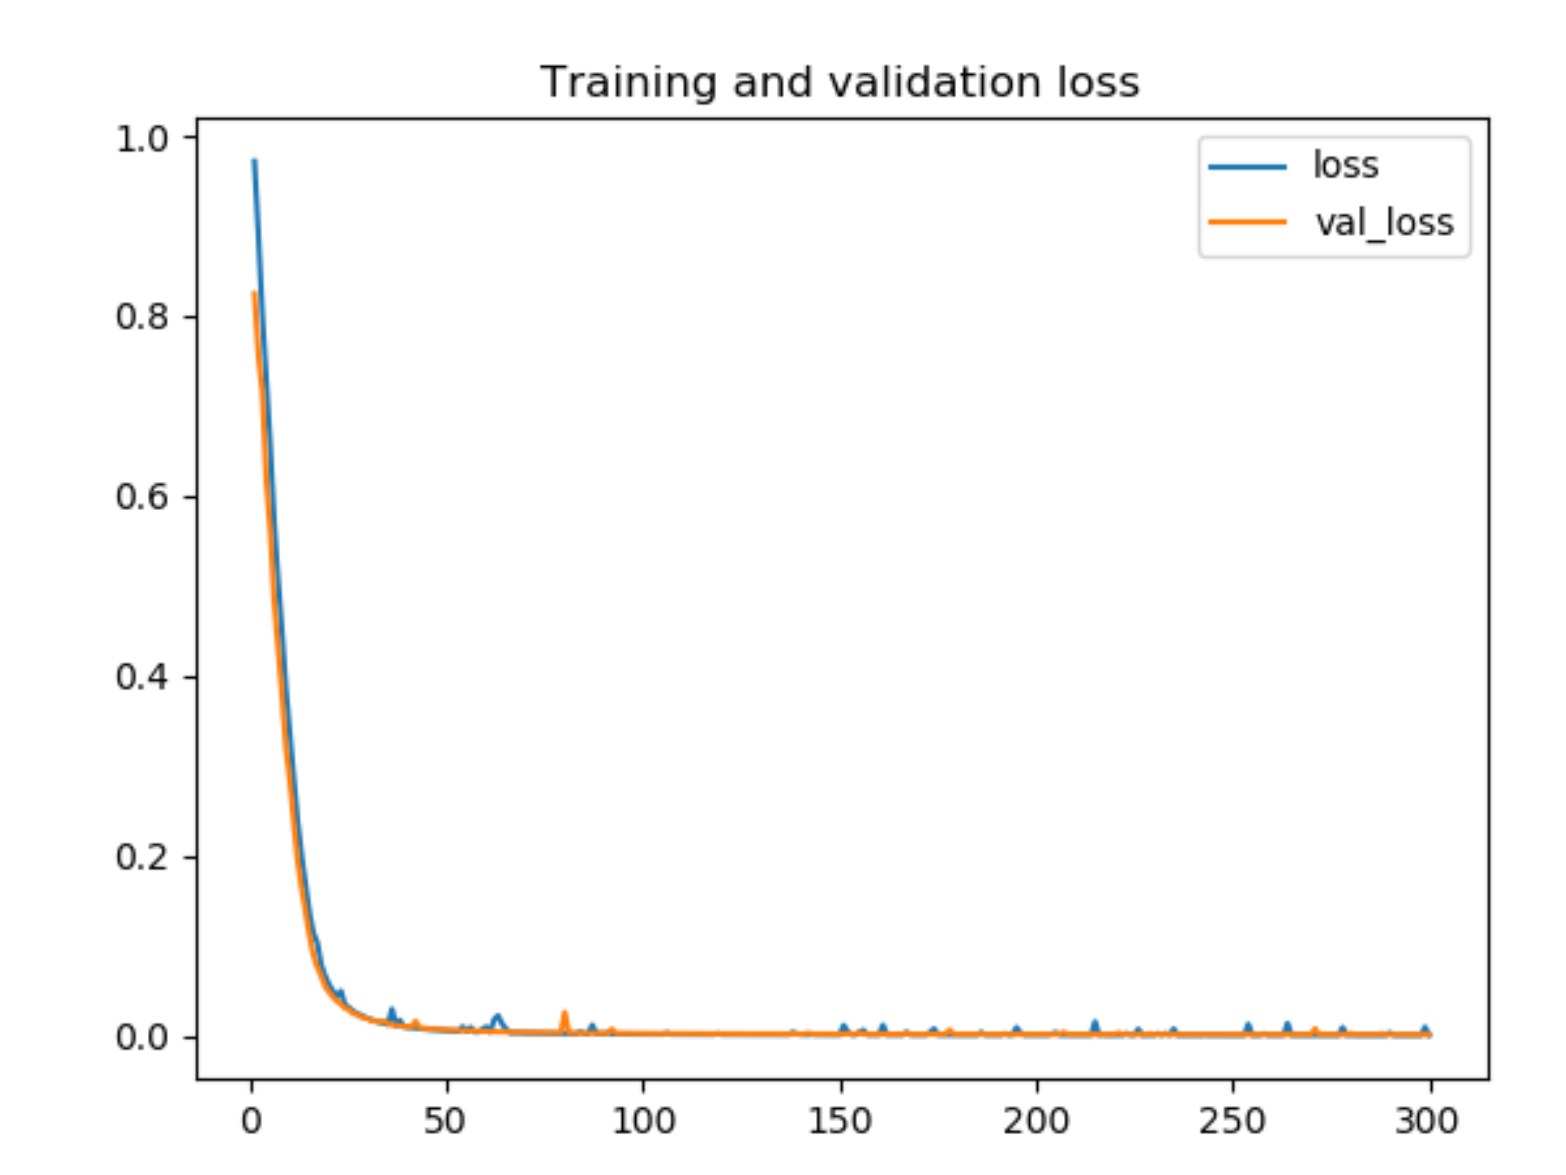
\includegraphics[width=\textwidth]{ResultsWind/windLog21.png}}
            \caption{Minimisation de la Loss MSE}
        \end{subfigure}
        \hfill
        \begin{subfigure}[t]{0.49\textwidth}
            \raisebox{-\height}{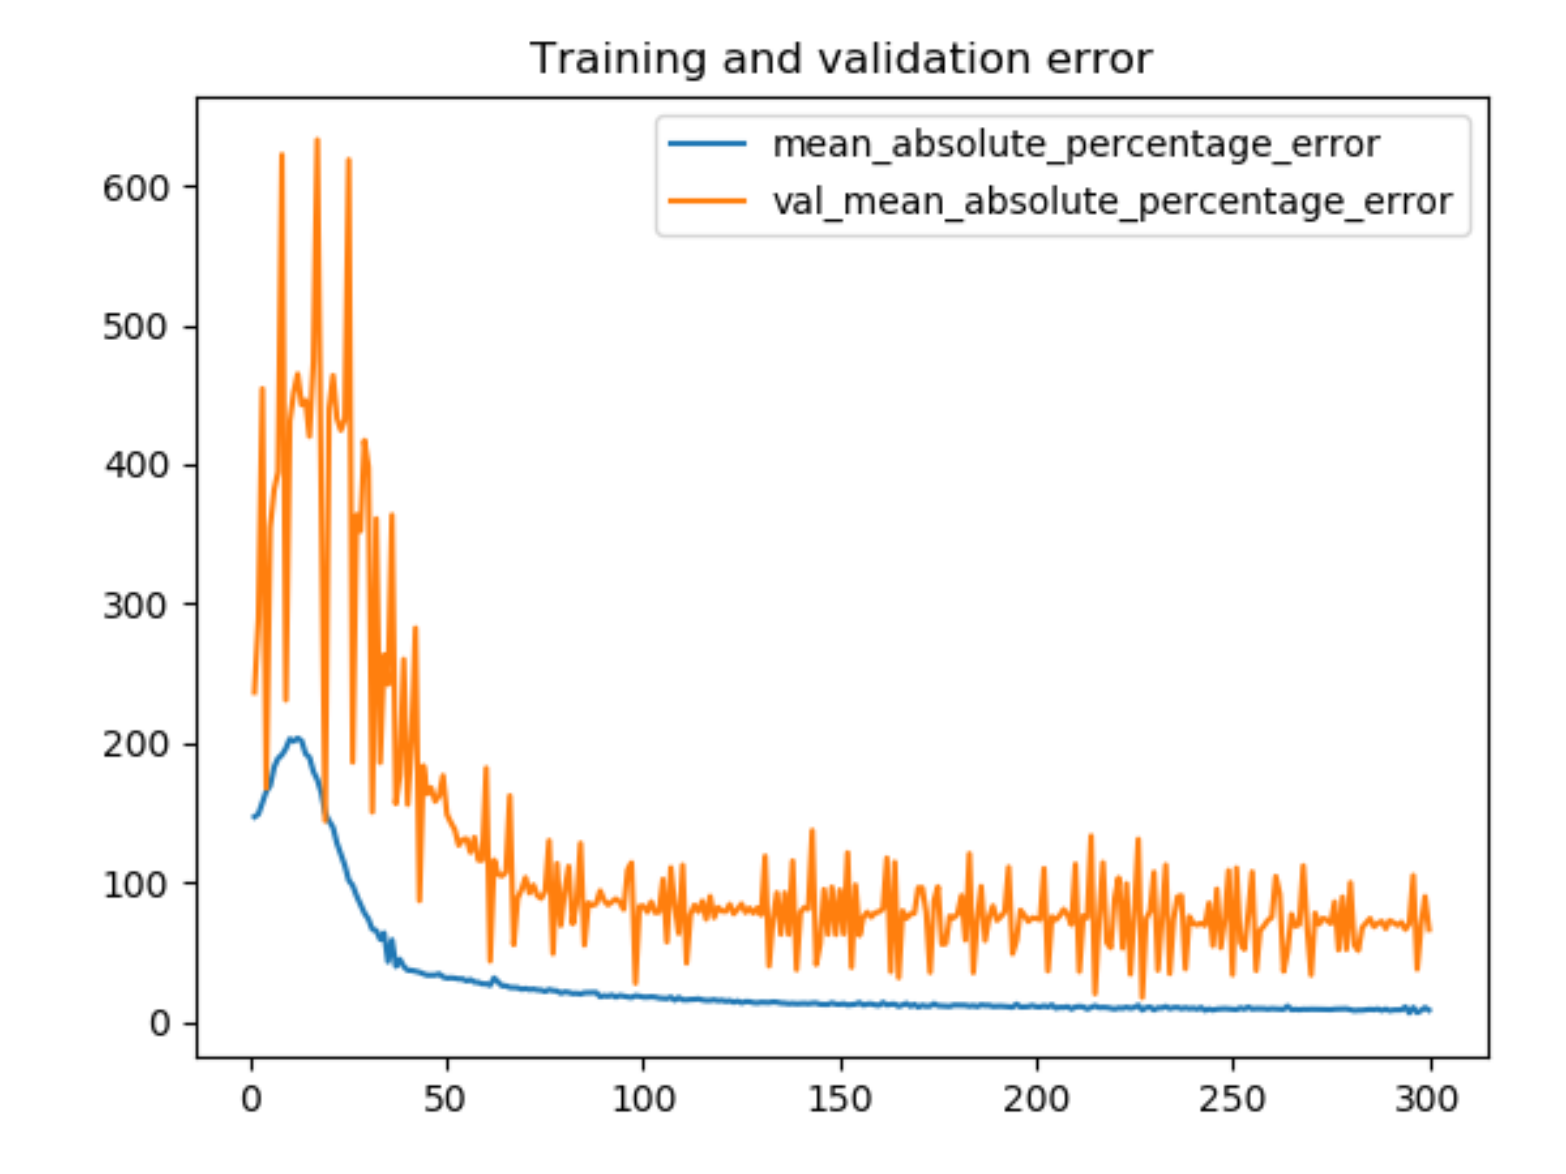
\includegraphics[width=\textwidth]{ResultsWind/windLog22.png}}
        \caption{Métrique MAPE}
    \end{subfigure}
        \caption{Performance du réseau : Reconstruction (Wind, Electricity Load)}
        \label{fig:test}
    \end{figure}

\section{Prédiction}
Cette tâche consiste à prédire une feature à t+x, x sup à 4, à partir des informations disponibles au temps t. On voit que dans le contexte de notre TP il peut être très intéressant pour l'entreprise fournisseuse de connaître en amont l'électricité générée. La loss reste la MSE, et la métrique reste la MAPE. On utilise un réseau de neurones pour cette tâche.\\
Après plusieurs essais, il semble être beaucoup plus difficile d'obtenir de bons résultats sur cette tâche, comparée à celle de reconstruction. L'idée qui nous vient est de donner plus de capacité au réseau par rapport à la tâche de reconstruction. Avec une meilleure capacité le réseau pourra mieux apprendre sa tâche de prédiction, car intuitivement cette tâche semble plus "complexe" que la tâche de reconstruction.\\Il faut également changer le nombre d'epoch, la tâche étant bien plus complexe à minimiser, on monte le nombre d'epoch à 500.\\\\
voici le réseau que l'on entraîne:
\begin{lstlisting}[frame=single]
        def create_model(w, c):
        """ Create a keras model
        # Arguments
            :param w: int, time dimension
            :param c: int, channel dimension
        # Returns
            :return: keras model
        """
        l_in = Input(shape=(w, c,))  
        
        @l_hidden_0 = Dense(1000, activation='relu')(l_in)
        l_hidden_1 = Dense(100, activation='relu')(l_hidden_0)
        l_hidden_2 = Dense(10, activation='relu')(l_hidden_1)
        l_hidden_out = Dense(1, activation='linear')(l_hidden_2)@
        l_out = Flatten()(l_hidden_out)

        return Model(l_in, l_out)
    \end{lstlisting}
Avec comme méta-paramètres : epoch=500, lr=1e-6, noise=3e-7, batch=120, chunk=12.
Voici les résultats que nous obtenons avec cette configuration :

\begin{figure}[H]
        \centering
        \begin{subfigure}[t]{0.49\textwidth}
            \raisebox{-\height}{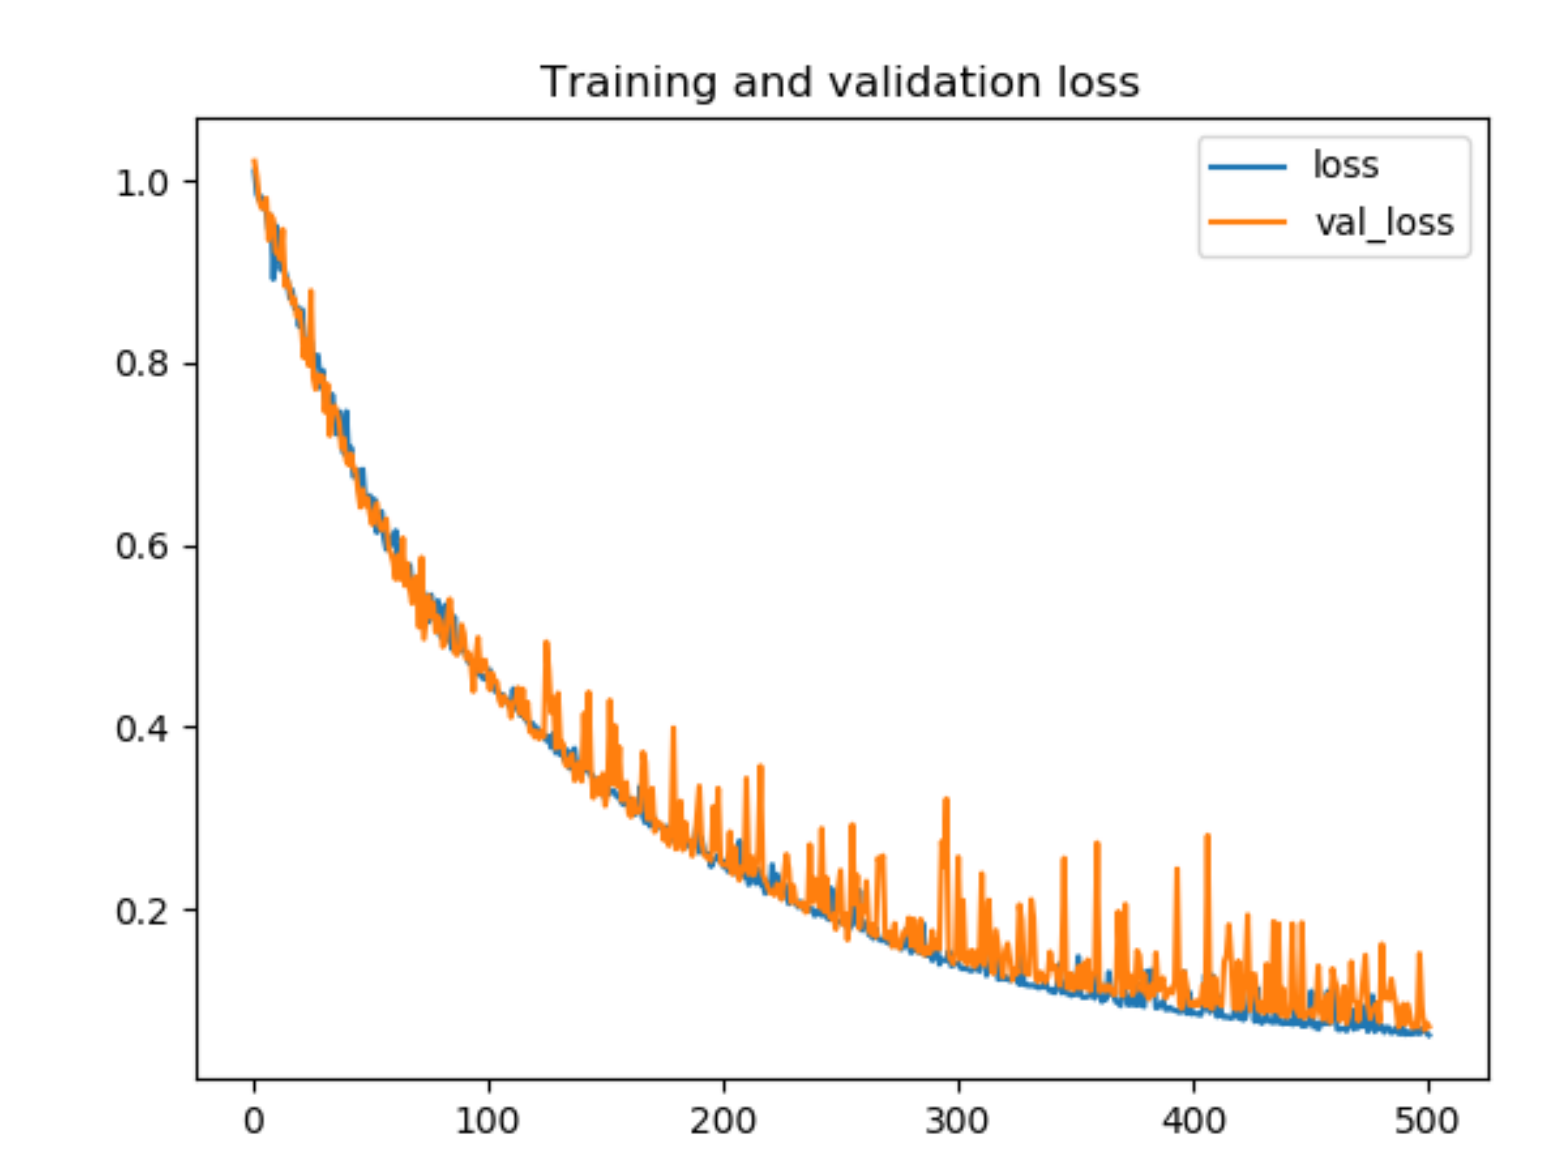
\includegraphics[width=\textwidth]{prediction/pred1.png}}
            \caption{Minimisation de la Loss MSE}
        \end{subfigure}
        \hfill
        \begin{subfigure}[t]{0.49\textwidth}
            \raisebox{-\height}{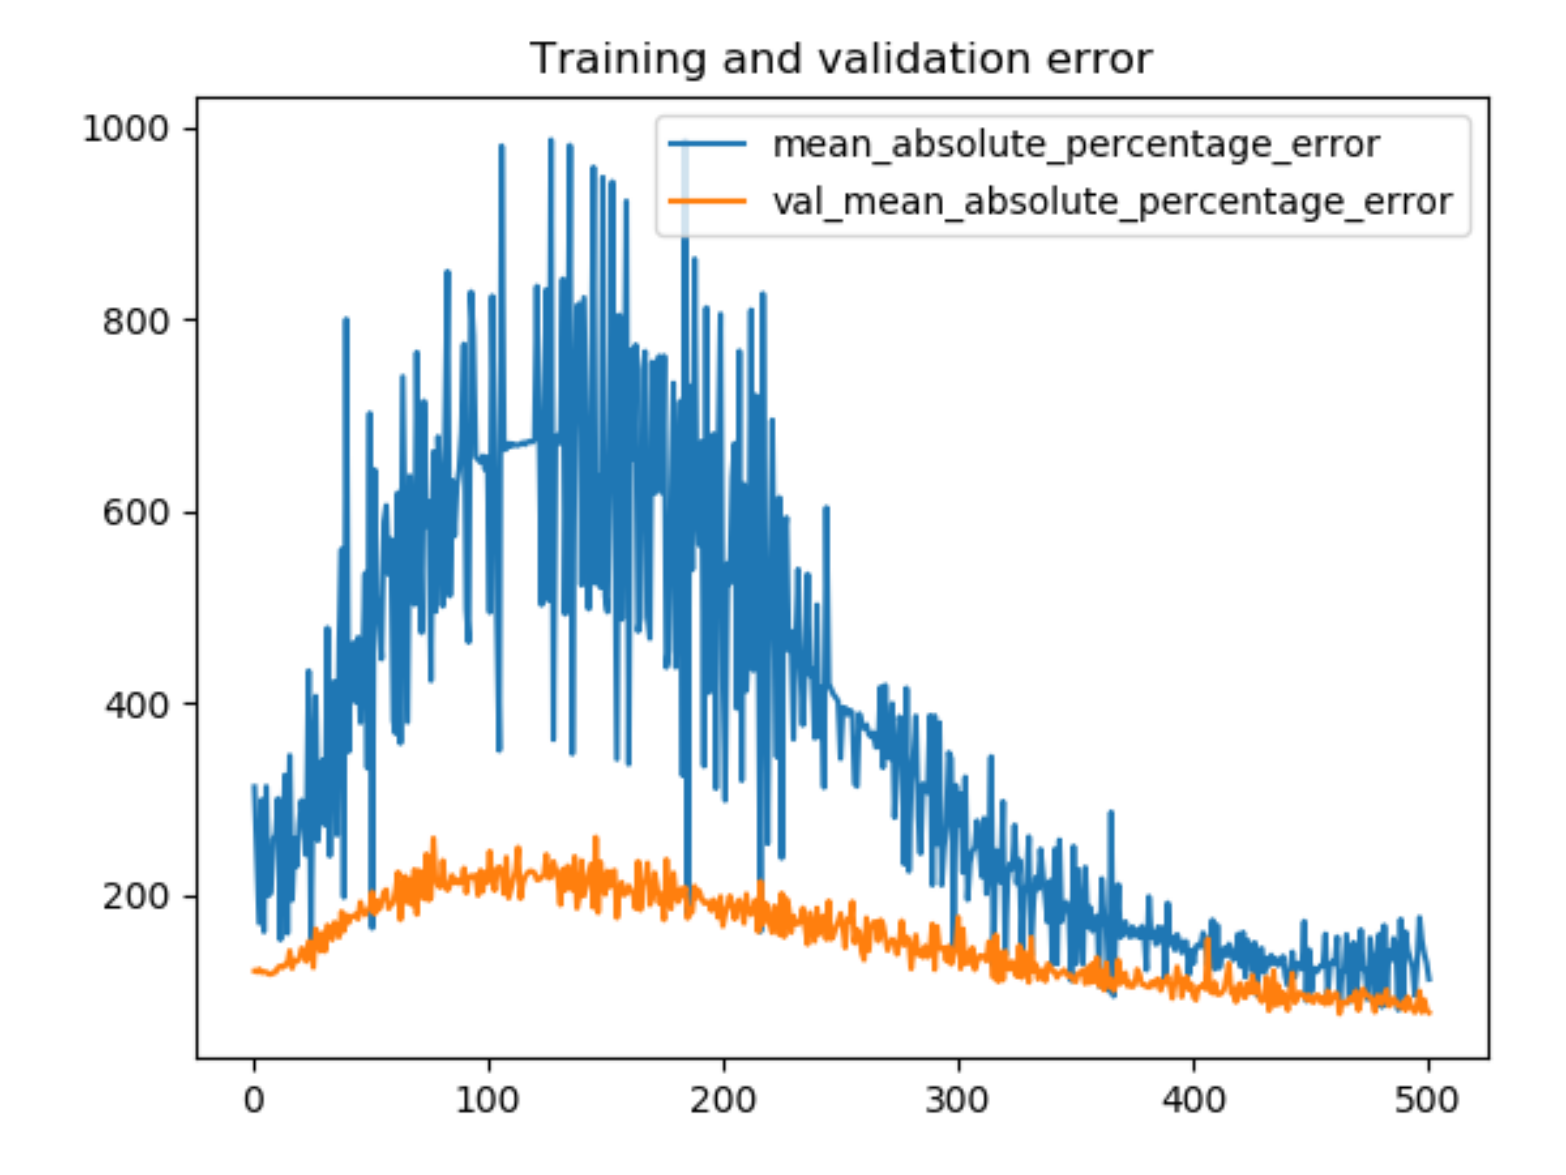
\includegraphics[width=\textwidth]{prediction/pred2.png}}
        \caption{Métrique MAPE}
    \end{subfigure}
        \caption{Performance du réseau : Prédiction (t+5) (Wind, Electricity Load)}
        \label{fig:test}
    \end{figure}
Au bout de 500 epoch on voit que le modèle possède une bonne performance, les métrique MAPE Train et Val convergent. La loss n'est en revanche pas complètement nulle pour les dataset Train et Val, idéalement il faudrait augmenter le nombre d'epoch (peut être 700 ?) pour obtenir une meilleure convergence.

\begin{figure}[H]
        \centering
        \begin{subfigure}[t]{0.49\textwidth}
            \raisebox{-\height}{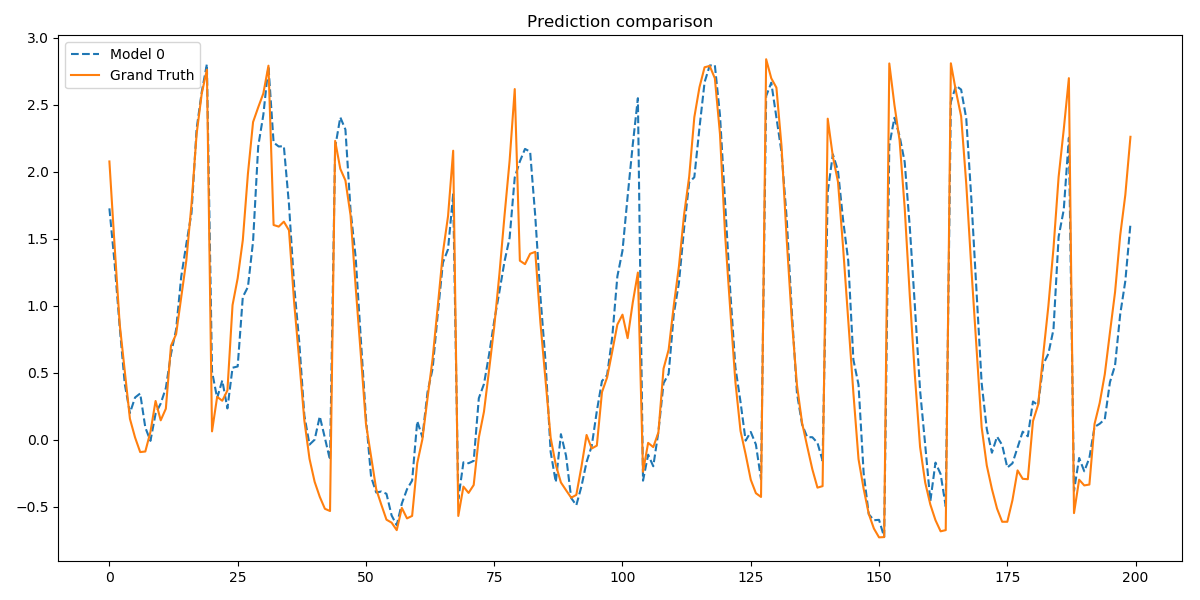
\includegraphics[width=\textwidth]{prediction/comparison_test_5.png}}
            \caption{Comparaison Test}
        \end{subfigure}
        \hfill
        \begin{subfigure}[t]{0.49\textwidth}
            \raisebox{-\height}{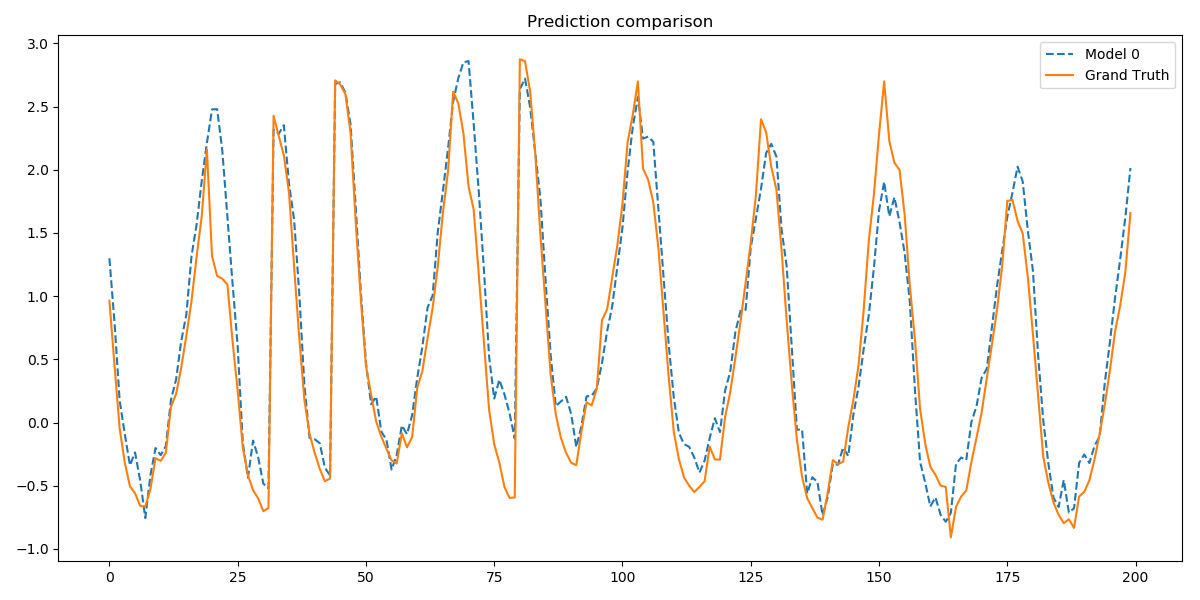
\includegraphics[width=\textwidth]{prediction/comparison_valid_5.png}}
        \caption{Comparaison Valid}
    \end{subfigure}
        \caption{Ecart de prédiction : Prédiction (t+5) (Wind, Electricity Load)}
        \label{fig:test}
    \end{figure}
L'écart de prédiction est beaucoup plus important que ce que l'on a obtenu avec la tâche précédente (Reconstruction), mais il reste acceptable.\\Ces résultats ne sont certes pas excellents mais ils consituent un bon premier modèle. Pour améliorer la prédiction plusieurs pistes d'améliorations sont possibles : augmenter la capacité, augmenter le nombre d'epoch, augmenter la taille du batch (meilleure approximation du gradient).
\section{Conclusion}
Nous avons réussi à proposer des modèles plus ou moins pertinents pour chaque use-case. Au fil de nos nombreuses expérimentations avec différents modèles, nous nous sommes vraiment rendus compte de la difficulté que représente la réalisation d'un "bon" modèle. Il y a beaucoup de paramètres à prendre en compte : la qualité des données, leur normalisation, la redondance, la corrélation, etc\ldots Une fois cette étape franchie, le second problème est le choix du modèle. Dans le cas d'un SVR (et autres modèles ``old-school``), le nombre de paramètres du modèle est assez limité, le cas d'un ANN est beaucoup plus complexe. Enfin, il faut choisir correctement les méta-paramètres (epoch, batch, chunk, learning rate, noise etc.). \\Tous ces choix sont autant de possibilités de se tromper : on se rend compte que "débugger" un ANN peut être particulièrement difficile. Dans notre TP, nous avons utilisé des modèles assez simples, mais dans le cas d'ANN beaucoup plus complexes (CNN, RNN, plusieurs dizaines de couches, des milliers de neuronnes etc.), il faut beaucoup d'expérience et d'intuition pour être capable de fournir des paramètres pertinents au modèle.


\end{document}